
%% 1-2 pages

\section{Related research}

To be able to design and develop the prototype of a visualization tool to help manage technical debt, previous work in relevant fields of research was reviewed.
This section presents and reviews the research from two main areas, technical debt management and information visualization, upon which this study builds.

\subsection{Technical Debt}
First described by Cunningham in 1992 \cite{cunningham_wycash_1992}, technical debt (TB) is a metaphor to financial debt and describes the common situation with increased development costs over time in software projects caused by poor software engineering practices \cite{tom_exploration_2013}.

Over time, the concept of technical debt gained in popularity and with that the scope of the metaphor was expanded to include any imperfection in the software lifecycle.
With this broader definition of technical debt, the need for strategies to monitor and manage the debt in a project are created.
Seaman and Guo, in the paper \textit{MEASURING AND MONITORING TECHNICAL DEBT}, proposes a "technical debt list" with "debt items" in order to monitor and keep track of instances of debt present in the project \cite{seaman_measuring_2011}.

The notion of a "debt item" will be used in this study to represent the debt in a project and present an overview to developers and other users of the proposed tool. 
The "debt item" described by Seaman and Guo includes a description of where in the system the debt is present and why the task needs to be payed off \cite{seaman_measuring_2011}.
In this study the concept is expanded to also include the type, or dimension of debt the item represents.

The idea of \textit{debt dimensions} was introduced by Tom et. al. in their exploration of the technical debt definition \cite{tom_exploration_2013}.
Through a multivocal literature review of the current technical debt literature as well as interviews with participants from industry, Tom et. al. proposed five distinct dimensions of technical debt; \textit{Code debt}, \textit{Design and architectural debt}, \textit{Environmental debt}, \textit{Knowledge distribution and documentation debt} and \textit{testing debt} \cite{tom_exploration_2013}.
Further, Tom et. al. also explores the factors that contributes to technical debt in projects and among them they identified the following main factors; \textit{Pragmatism}, \textit{Prioritization}, \textit{Process}, \textit{Attitudes} and \textit{Ignorance} \cite{tom_exploration_2013}.

Of special interest to this study are \textit{Prioritization}, \textit{Process} and \textit{Attitudes} since these are factors that are addressable through a visualization tool.
Tom et. al. writes, "The visibility of all forms of technical debt decreases when poor communication and collaboration processes are in place, making it easier for debt to accumulate without being noticed." \cite{tom_exploration_2013} suggesting that visibility and communication are key to establishing a successful technical debt management process.

Worth noting when when dealing with technical debt is that, even though concept in many ways are associated with negative effects, in some cases, taking on technical debt can be a strategic short term decision in order to reach a critical deadline in time.
However, if not properly managed the debt can be costly by decreasing development velocity and increasing maintenance costs \cite{seaman_using_2012}.

\subsection{Information Visualization}

The core of information visualizations are the mapping of data and intent to visual representations.
Although there are many different techniques used in the field, this central process of visualizations can be described by the \textit{Reference model for visualization} by Card et al. presented in figure \ref{fig:vizprocess} \cite{card_readings_1999}. 
This common reference model is helpful in order to analyze and compare the different techniques as seen in the taxonomy proposed by Chi based on model by Card et al. \cite{chi_taxonomy_2000}.

\begin{figure}[t]
  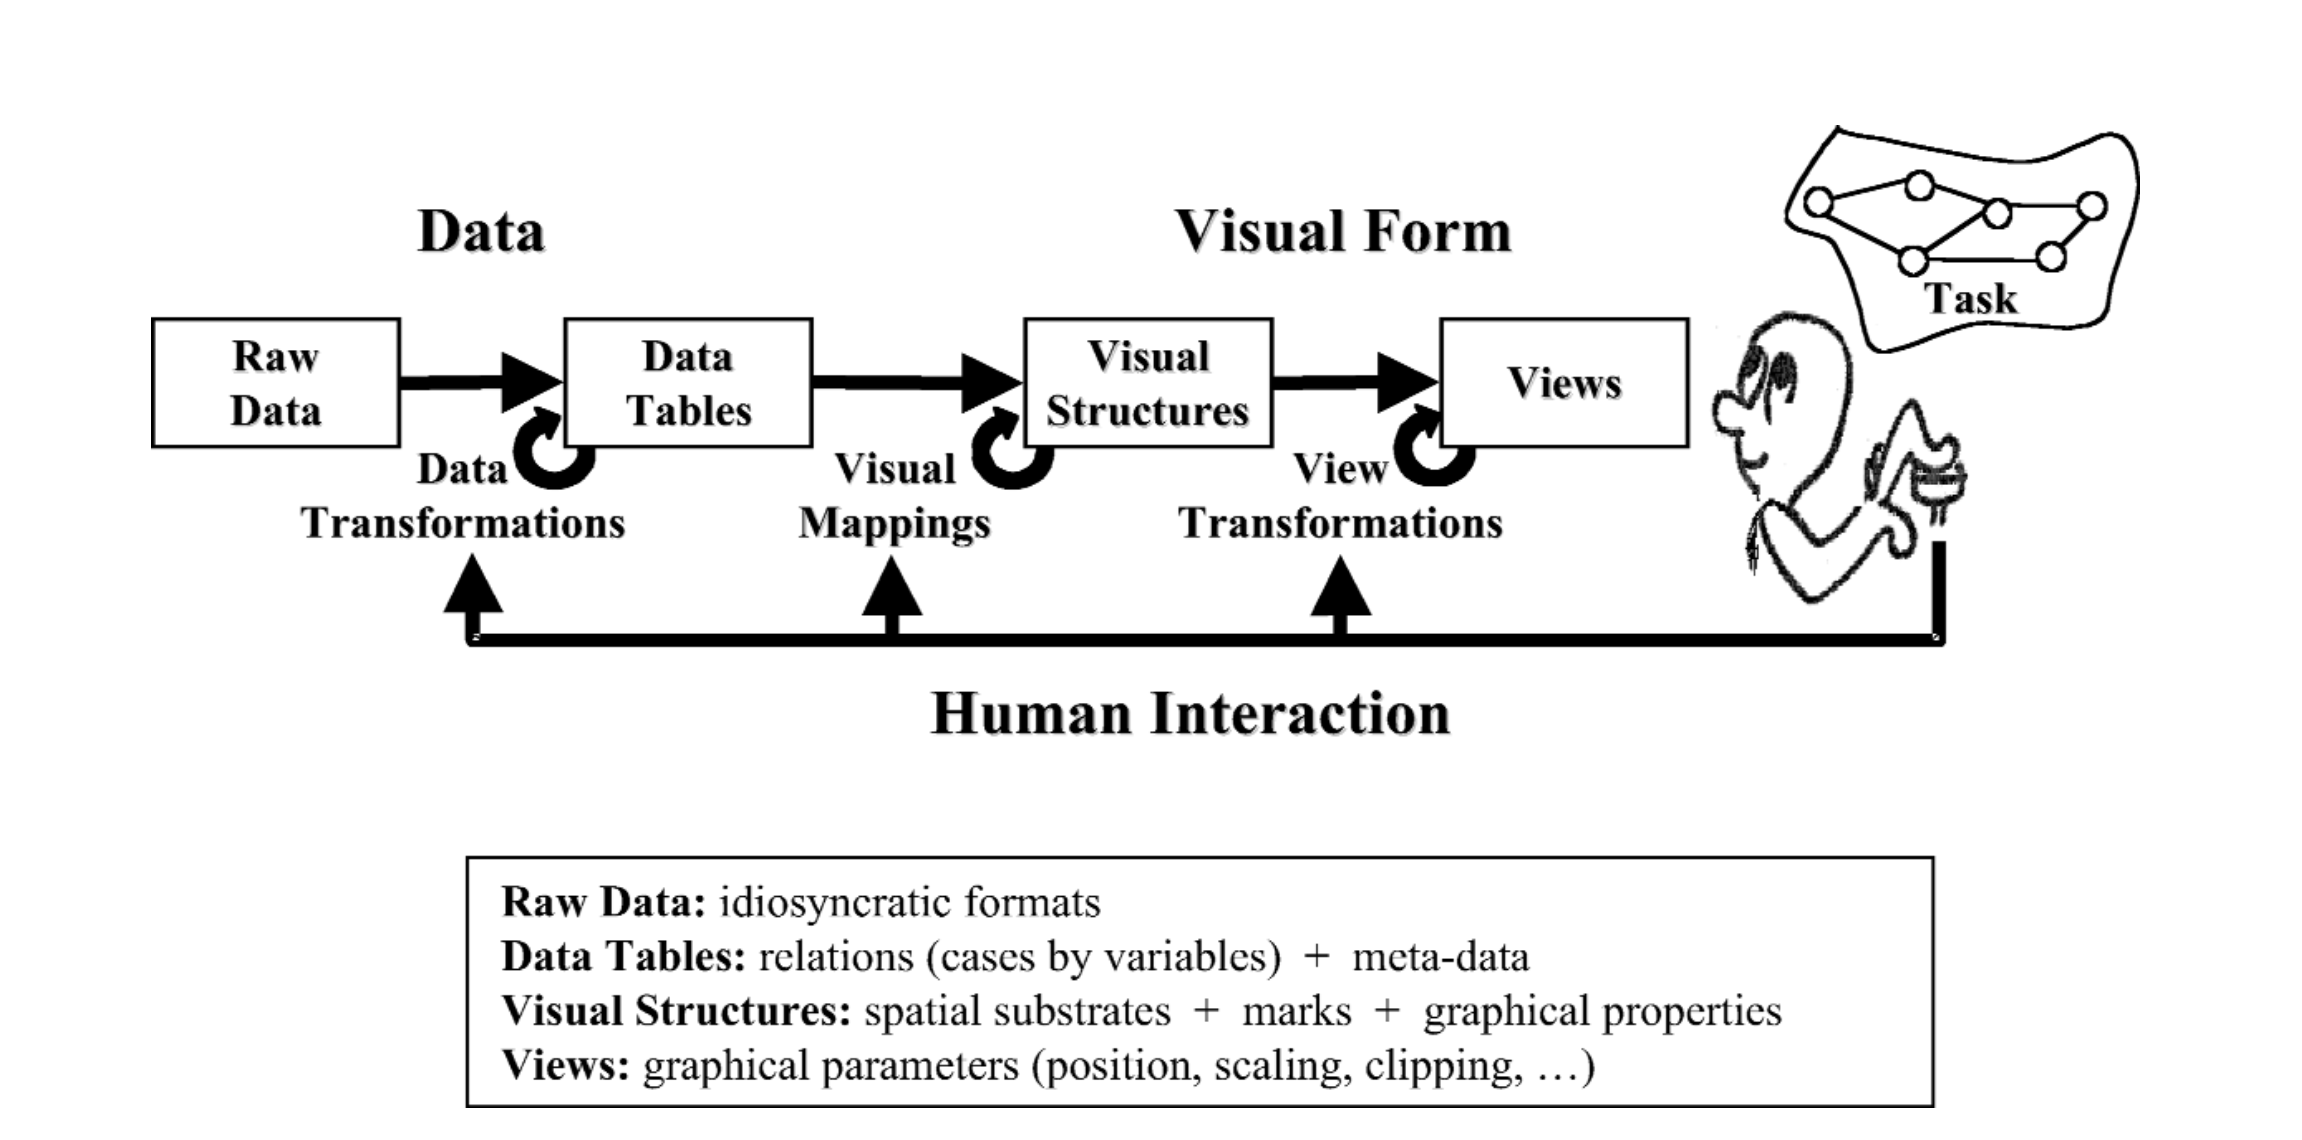
\includegraphics[width=\columnwidth]{VisualizationProcess}
  \Description{Chart over the Reference model for visualization by Card et al. 1999}
  \caption[Reference model for visualization]{Reference model for visualization by Card et al. 1999 \cite{card_readings_1999}}.
  \label{fig:vizprocess}
  \centering
\end{figure}

The raw data can take many forms which can be classified intro three main categories based on its properties, \textit{nominal data} is simple data with some sort of label but no quantitative value, \textit{ordinal data} can be ranked according to some attribute and \textit{quantitative data} which support arithmetic operations \cite{card_structure_1997}.
In this study, the source code of a software project is visualized.
The source code is a collection of files and folders that translates into a hierarchical data structure with nodes where each node can contain, or like to, a set of child nodes generating a tree-structure.
Hierarchies are closely related to network data structures, with the main difference being that hierarchies does not contain any loops within the connections \cite{spence_information_2014}.
Techniques to visualize hierarchies has been a heavily researched topic going far back, and there are multiple approaches and techniques to consider which can be divided into two separate groups, according to a survey of the design space by Schultz et. al. \cite{schulz_design_2011}. 
Explicit tree visualizations are visual representations where the relations between nodes are shown with explicit lines or arcs, whereas implicit tree visualizations uses techniques such as adjacency and encapsulation to represent the relationship between parent and child nodes \cite{schulz_design_2011}.